\documentclass[prl,twocolumn]{revtex4-1}

\usepackage{graphicx}
\usepackage{color}
\usepackage{latexsym,amsmath}
\usepackage{amsfonts}
\usepackage{caption}

\definecolor{linkcolor}{rgb}{1.0,0.647,0.0} %hyperlink
\usepackage[pdftex,colorlinks=true, pdfstartview=FitV, linkcolor= linkcolor, citecolor= linkcolor, urlcolor= linkcolor, hyperindex=true,hyperfigures=true]{hyperref} %hyperlink%

\usepackage{enumitem}
\setlist[itemize]{leftmargin=*}


\setcounter{secnumdepth}{2}

\renewcommand{\thesection}{\arabic{section}}
\renewcommand{\theequation}{\thesection.\arabic{equation}}

\makeatletter
\@addtoreset{equation}{section} % Reset equation counter at each section
\makeatother

\begin{document}

\title{Quantum Optics and Laser, Lab2 - Grangier-Roger-Aspect experiment}



\author{Calandra Buonaura Lorenzo}

\date{\today}


\begin{abstract}

In this experiment, we explore the particle-like properties of light by replicating a version of the Grangier-Roger-Aspect test. Our objective is to demonstrate the quantized nature of light and verify that single photons do not simultaneously trigger multiple detectors, thus highlighting the indivisibility of photons. By using a beam splitter and two photodetectors, we examine the photon statistics and confirm that, contrary to classical expectations, photons do not split but instead exhibit clear particle-like behavior, aligning with quantum mechanical predictions. Furthermore, we take advantage of the intrinsic randomness of quantum events by implementing a Quantum Random Number Generator leveraging the arrival times of transmitted and reflected photons.
\end{abstract}

\maketitle

\section{Introduction}
The Grangier-Roger-Aspect (GRA) experiment stands as a landmark investigation into the fundamental nature of light and its quantum properties; designed in the 1980s, it aimed to directly test the principles of quantum mechanics by exploring the phenomenon of single-photon interference and nonlocality. In particular, this experiment used a beam splitter to probe how individual photons would behave when encountering a choice between two paths — reflected or transmitted. Classical physics might predict that light (considered a wave), even in weak beams, could split across both paths, leading to simultaneous detections in both channels; however, GRA’s results demonstrated that photons behave as indivisible quantum particles, showing up in only one detector at a time~\cite{pap1}. 

This all-or-nothing behavior, called ``anticorrelation'' was essential for confirming that light’s behavior cannot be fully explained by classical wave models: individual photons, in fact, exhibit probabilistic outcomes, with detection events occurring in discrete, singular units rather than as a continuous wave. These findings helped validate the idea that light has an intrinsic quantized nature, acting as individual quanta or particles when subjected to measurement, thus confirming the double nature of light, the particle-wave dualism.

In our experiment, we first produce photon couples thanks to a non-linear optical effect called Spontaneous Parametric Down Conversion (SPDC): thanks to this effect, we can use one of the two photon as an ``herald photon'' for the other, which is then the one analyzed. Then, we study the photon arrival times after the beam splitter, in both the transmitted and the reflected channel, leveraging a coherent light source; by studying the distribution of these arrival times, we aim to investigate the discrete and inherently random nature of photon detection events.

Additionally, we utilize photon arrival times to implement a Quantum Random Number Generator (QRNG), which is made possible to the intrinsic probabilistic nature of photon detection. By recording the exact arrival times of photons in the transmitted channel, we produce a sequence of random numbers; the randomness is intrinsic in the arrival times due to the randomness of the spontaneous photon emission in the crystal and the randomness of the number of detected photons (for a coherent state of light). Unlike classical methods, which rely on deterministic algorithms and may exhibit biases or patterns, this quantum-derived procedure provides an ideal basis for applications in secure communications, cryptographic systems, and high-fidelity simulations.

\section{Theoretical framework}
In quantum optics experiments, single-photon phenomena are central to understanding the intrinsic probabilistic nature of quantum mechanics; the Grangier-Roger-Aspect (GRA) experiment exploits these concepts to probe the behavior of individual photons and to test the foundations of quantum mechanics.

\subsection{Malus Law}
Malus' law describes how the intensity of a linearly polarized light beam changes as it passes through a polarizing filter, which is used to module light intensity in quantum optics experiment and polarize light along one direction. When a beam of light with an initial intensity $I_0$ and polarization angle $\theta$ passes through a polarizer oriented at an angle $\alpha$ relative to the light's polarization direction, the transmitted intensity $I$ is given by:

\begin{equation}
    I = I_0 \cos^2(\theta - \alpha)
    \label{eq:malus_law}
\end{equation}

where $I_0$ is the initial intensity of the incoming light before the polarizer, $\theta$ is the angle of the initial polarization direction of the light and $\alpha$ is the angle of the transmission axis of the polarizer~\cite{pap2}. When the angle $\theta - \alpha$ is $0^\circ$, the transmitted intensity is at its maximum and equals $I_0$, while when the angle is $90^\circ$, the transmitted intensity becomes zero, as the light is completely blocked by the polarizer.

\begin{figure*}[!t]
    \centering
    \includegraphics[width=0.8\linewidth]{Images/SPDC_scheme.png}
    \caption{(a) Schematic illustration of the process of spontaneous parametric down-conversion (SPDC). (b) Energy-level description and (c) wavevector description of the process~\cite{pap3}.}
    \label{fig:SPDC_scheme}
\end{figure*}

\subsection{Spontaneous Parametric Down Conversion (SPDC)}
\label{sec:SPDC}

Spontaneous Parametric Down-Conversion (SPDC) is a quantum optical process in which a single photon from a high-energy beam (known as the \textit{pump photon}) spontaneously decays into two lower-energy photons, known as \textit{signal} and \textit{idler} photons (depicted in Figure~\ref{fig:SPDC_scheme})~\cite{pap3}. This phenomenon is a direct result of the nonlinear interaction between the pump photon and a nonlinear crystal, often engineered to facilitate such conversions. 
In a nonlinear medium with second-order susceptibility $\chi^{(2)}$, the electric polarization $\vec{P}$ of the medium can be described as:
%
\begin{equation}
\vec{P} = \varepsilon_0 \chi^{(2)} \vec{E}^2,
\end{equation}
%
where $\vec{E}$ is the electric field of the incident pump photon, and $\varepsilon_0$ is the permittivity of free space.

During SPDC, energy conservation and momentum conservation, or phase-matching, must be satisfied:
%
\begin{equation}
    \hbar \omega_p = \hbar \omega_s + \hbar \omega_i,
\end{equation}
\begin{equation}
    \vec{k}_p = \vec{k}_s + \vec{k}_i,
\end{equation}
%
where $\omega_p$, $\omega_s$, and $\omega_i$ are the angular frequencies of the pump, signal, and idler photons, respectively, and $\vec{k}_p$, $\vec{k}_s$, and $\vec{k}_i$ are their respective wave vectors. These relations ensure that the energy and momentum of the generated photons match that of the pump photon~\cite{pap3}. When the frequencies $\omega_s$, and $\omega_i$ are equal, we have \textit{degenerate SPDC}: in this case the pump photon is split into two photons with identical frequencies and equal energy, each having exactly half the frequency of the pump photon:
\begin{equation}
    \omega_p = 2 \omega_s = 2 \omega_i    
\end{equation}

This situation arises under specific phase-matching conditions, typically achieved by carefully choosing the properties of the nonlinear crystal (such as its temperature, orientation, and type) and the pump wavelength.

\begin{figure}[!b]
    \centering
    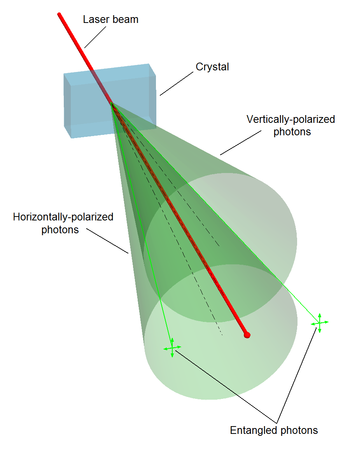
\includegraphics[width=0.7\linewidth]{Images/SPDC_cones.png}
    \caption{Type II SPDC: a non-linear crystal produces couples of entangled photons with opposite polarization.}
    \label{fig:SPDC_cones}
\end{figure}

The photon pairs generated through SPDC are typically entangled in polarization, momentum, or frequency; usually, the crystal is engineered to produce couples of entangles photon with orthogonal polarizations (type II SPDC, the one used in the experiment), which are useful in quantum information and quantum communication experiments. This is possible because the two emitted photons each follow a cone of emission with an angle determined by the energy and momentum conservation laws previously presented; in type II SPDC, the signal and idler photons are emitted on overlapping but distinct cones, creating intersection regions known as ``zones of coincidence'', where we can collect photons that are polarization-entangled (as seen in Figure~\ref{fig:SPDC_cones}). 

In our experiment, we leverage the fact that, during this process, a pair of correlated photons is always produced simultaneously. One of these photons acts as a "herald" for the other (which is the one which instead will go through the beam splitter), signaling its presence and arrival time to the other detector; by detecting the herald photon, we effectively announce the presence of its paired photon, allowing us to synchronize and measure the exact timing of the paired photon's arrival with high accuracy. This heralding technique is crucial, because it allows us to filter out background noise and other unrelated detection events, ensuring that we only record true, correlated photon pairs.

\subsection{Beam-splitter}
\label{sec:beam_splitter}
In classical optics, a beam splitter is typically modeled as an optical device that divides an incoming light beam into two separate paths. Assuming an ideal, lossless 50:50 beam splitter, the amplitude of the incident electric field \( E_{\text{in}} \) is split equally between the transmitted and reflected paths. Thus, for a 50:50 beam splitter, the relationship between the input and output fields can be described by:
%
\begin{equation}
    E_{\text{t}} = \frac{1}{\sqrt{2}} E_{\text{in}}, \quad E_{\text{r}} = \frac{i}{\sqrt{2}} E_{\text{in}},
\end{equation}
%
where \( i \) represents a phase shift of \(\pi/2\) introduced upon reflection. This phase shift is a characteristic of the beam splitter and results in destructive interference when two beams interfere on the output ports of the device. The intensities of the transmitted and reflected beams, given by \( I \propto |E|^2 \), are each half of the input intensity \( I_{\text{in}} \)~\cite{pap2}.

Now, given an experiment about single photons and photodetectors, we can describe classically the behavior of the beam-splitter having a look to the counts that each detector has. Considering a ``triggered experiment'' like this one involving SPDC, we can define the detection probabilities as:
%
\begin{equation}
    p_t = \frac{N_t}{N} \qquad p_r = \frac{N_r}{N} \qquad p_c = \frac{N_c}{N}
\end{equation}
%
where $p_t$ is the probability of the photon being transmitted, $p_r$ is the probability of the photon being reflected and $p_c$ is the probability for a coincidence. It can be proven that, for a classical description, it holds:
%
\begin{equation}
    p_c \geq p_r \: p_t
\end{equation}
%
or equivalently
%
\begin{equation}
    \alpha \geq 1, \qquad \text{with} \:\: \alpha = \frac{p_c}{p_r \: p_t} = \frac{N_c \: N}{N_r \: N_t}
    \label{eq:alpha}
\end{equation}
%
These inequalities mean clearly that the classical coincidence probability pc is always greater than the \textit{accidental coincidence} probability, which is equal to $p_r\:p_t$. The violation of Equation~\eqref{eq:alpha} thus gives an anticorrelation criterion, for characterizing a nonclassical behaviour~\cite{pap1}.

But why would nonclassical behaviour arise? Well, simply because the classical model doesn't take into account photon indivisibility, treating light beam (also at a very low intensity) as waves. Due to photon indivisibility, which is a properly quantum effect, we have that each photon can be either reflected or transmitted; single photons are not splitted. From this simple consideration, we expect a very low value for $p_c$, which will lead to the violation of Equation ~\eqref{eq:alpha}.



\subsection{Quantum Random Number Generator}
\label{sec:qrng_theory}
We can leverage coherent light to build a quantum random generator; the main idea is based on Eisenberg's principle, which states that the product between the uncertainty over time and the uncertainty over energy is always greater than a finite value, meaning that we can't know with infinite precision both energy and time of arrival. We can apply this concept to the photon absorbed by the photodetector: the more precisely the energy of the photon is known (as is the case in a coherent light), the less precisely its arrival time can be predicted. This uncertainty in the time of detection, combined with the probabilistic nature of photon emission, ensures that each photon’s detection is independent of the others and inherently unpredictable.

In particular, for coherent light, photon arrivals follow a Poisson process, where the time intervals between consecutive photon detections are exponentially distributed. The probability density function for the time interval $\Delta T$ between photon arrivals is given by:
%
\begin{equation}
    \label{eq:geometric_distribution}
    f(\Delta T) = \lambda e^{-\lambda \Delta T}
\end{equation}
%
where $\lambda$ represents the average photon detection rate. This exponential distribution arises because, as already pointed out, the emission of photons in a coherent state occurs without any underlying regular pattern or periodicity. In fact, quantum mechanics dictates that each photon has a certain probability of being detected at any given moment, but the precise timing of each event cannot be predicted, which constitutes the perfect ingredient for our quantum random number generator.

But how can we arrive to the QRNG from the arrival time? We need to convert these random times in bit: we can do it considering only the photons arrived in either the transmitted or the reflected channel and assigning them a 0 or a 1 value, respectively. After this first step we can group the bits into blocks of 8 to form bytes and convert them to decimal to create our sequence of random numbers: every number in $[0, 255]$ should have the same probability of occurrence, i.e. the resulting byte distribution is expected to be uniform. In order to see if the randomness of the sequence is real we need to introduce some tests that take into account the correlation between values in the sequence, which are explained in Appendix~\ref{sec:appendix_random}.


\section{Apparatus}
\begin{figure}[!b]
    \centering
    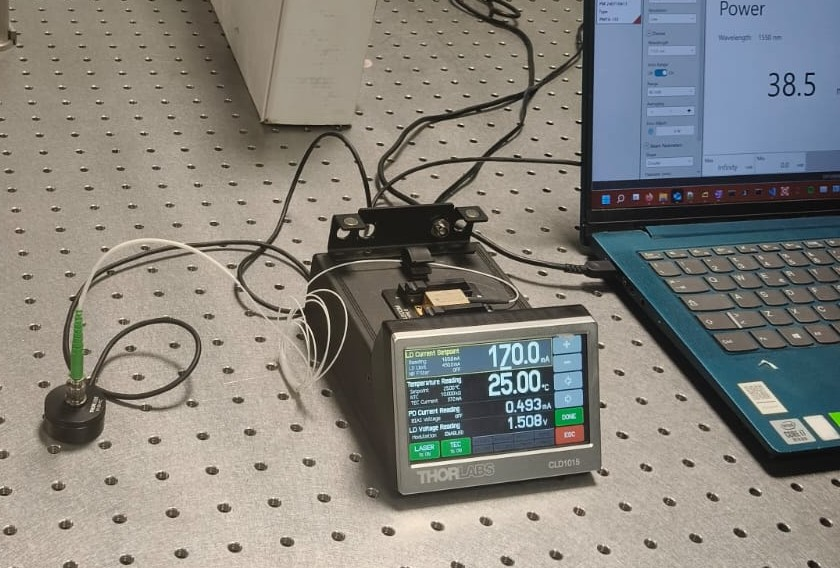
\includegraphics[width=\linewidth]{Images/setup.jpg}
    \caption{Experimental setup, where numbers correspond to the different components explained in the text.}
    \label{fig:setup}
\end{figure}

The setup for this experiment is pretty simple; the main ingredients are a laser, some optical elements (like lenses and polarizers), the non-linear crystal and a single photon detector. We can see a picture of the whole setup in Figure~\ref{fig:setup}. Obviously, every component has a specific role in the experiment, which is explained in the following:

\begin{enumerate}
    \item \textbf{Gas Tube Laser:} The light source in this experiment is a gas laser, which produces a highly monochromatic (purplish, $\lambda = 405 nm$) and phase-stable beam, ideal for experiments requiring precise control over the light’s properties (coherent light).
    \item \textbf{Mirrors and polarizers:} A system of mirror and polarizers is placed after the laser beam, to redirect and reduce the intensity of the beam (following Equation~\eqref{eq:malus_law}). The last element of this set is a collimator which takes the divergent light beam and converts it into a parallel beam before it hits the crystal.
    \item \textbf{Non-linear crystal:} The third element of the setup is the non-linear crystal responsible for the production of the couples of photons (SPDC, see Section~\ref{sec:SPDC}). In this experiment we used a BBO crystal (beta barium borate, with the chemical formula $\text{BaB}_2\text{O}_4$), which exhibits strong non-linear effects (as requested).
    \item \textbf{Pinholes:} These elements are essential for spatial filtering and controlling light beams; thanks to these we can select which part of the two non-collinear beam cones we want to see. Thus, by allowing only specific paths of photons to pass, pinholes can reduce background noise and enhance the visibility of quantum interference patterns (important in entanglement experiments). 
    \item \textbf{Mirrors and polarizers:} Another system of mirrors and polarizers is used to direct towards two different regions the herald photon beam and the other photon beam, in order to improve the detection performance.
    \item \textbf{Beam splitter:} This element is obviously present in only one of the paths and is used to divide the photons in transmitted and reflected, following the idea explained in Section~\ref{sec:beam_splitter}. In this experiment we used a polarized beam-splitter, which splits photon based on their polarization (either vertical or horizontal).
    \item \textbf{Collimators:} The beams then are collected by three collimators, which collect the divergent light beams and converts it into parallel beams before coupling it into an optical fiber, ensuring that the light entering the fiber is properly aligned and maintains the necessary intensity for efficient transmission.
    \item \textbf{Optical Fiber:} The optical fiber then transmits the collimated light from the experimental setup to the photon counting system with minimal loss, keeping it isolated from external disturbances.
    \item \textbf{Single Photon Counting Modules (SPCM):} Then, the beams enter the three single-photon counters (SPAD, Single-Photon Avalanche Diode), which generate a peak of current when a photon is detected, a ``click". An important note to be done is about the working condition this device should be used in: due to its high absorbance, all not necessary light sources must be turned off, to reduce background-noise pollution of the signal and the device should be positioned under a black cloth to reduce even more unwanted clicks.
    \item \textbf{Time Tagger:} The arrival times are recorded thanks to the time tagger, which is an electronic device that logs the exact time at which each photon detection event occurs. The time resolution of the tagger is typically in the nanosecond range, ensuring precise timestamping of each photon event; we must also underline that the time tags of arrival are registered in ``machine units" of  $80.955$ ps. Three channels of the Time Tagger are used, to account for the three SPAD used: Channel 1 is for the herald photons, Channel 2 for the transmitted and Channel 3 for the reflected.
    \item \textbf{Computer:} Finally, we use the computer to process the data collected by the time tagger and produce the datasets that are used for the analysis of the two quantum state distributions.
\end{enumerate}

All components are securely mounted on an optical table, providing a stable and vibration-isolated environment. This setup minimizes external disturbances, such as mechanical vibrations or air currents, which could introduce significant noise into the photon detection process, falsifying the result of the experiment.

\section{Results}
\subsection{Malus' Law}
First of all, we proceed at verifying Malus' law, analyzing the transmitted photon number as the angle of the polarizer varies, in order to see whether if Equation~\eqref{eq:malus_law} is respected. Figure~\ref{fig:malus_law} depicts the data and the corresponding fit using the function:
%
\begin{equation}
    f(\theta) = a\:\cos^2(b\:\theta + c)
\end{equation}
%
As it's clear from the picture, we obtain a very good fit, with a percentage RMSE (Root Mean Square Error) of 0.4\%. From the fit we can obtain the best values for the parameters; the most informative about our setup are b and c, which are the parameters regarding the angular part, while we can leave out from the discussion the amplitude (which is in line with what expected). The fit yields the following results: $b = 0.998 \pm 0.002$ and $c = (-25.890 \pm 0.003)^\circ \:$. As we can see, the value of $b$ is in perfect agreement with the one expected from Equation~\eqref{eq:malus_law} ($b=1$); on the other hand, the value of $c$ represents the angle of the transmission axis of the polarizer, which indicates that we'll have a maximum transmission for $\alpha_1 = -25.89^\circ$ and a minimum for $\alpha_2 = \alpha_1 + 45^\circ$.

\begin{figure}[!b]
    \centering
    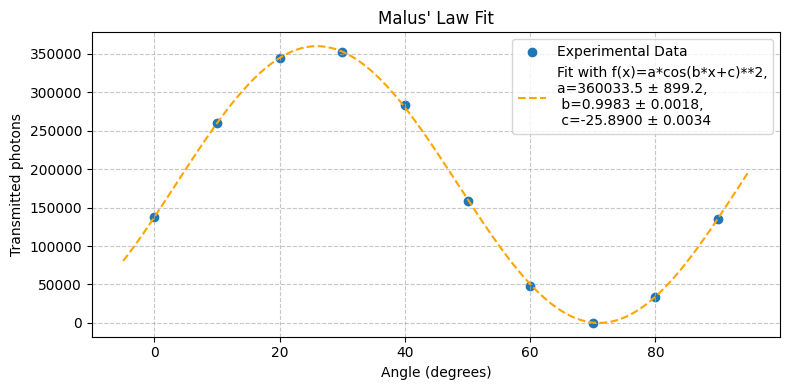
\includegraphics[width=\linewidth]{Images/malus_law.png}
    \caption{Polarizers modulate intensity following Malus' law (Equation~\eqref{eq:malus_law}).}
    \label{fig:malus_law}
\end{figure}

\subsection{GRA experiment}
First of all we can take a very fast look to the whole dataset; Figure~\ref{fig:photon_arrivals} depicts the photon counts at progressing time (count/5sec) for the whole period of the detection. Already from this simple histogram, we can see that herald photons are around double in number w.r.t. transmitted and reflected photons, as expected (because of every couple of photons one is the herald and on is transmitted OR reflected). We can also notice that reflected photons are a little less than transmitted photons, probably due to the beam splitter not being a perfect 50:50 beam splitter, but this doesn't constitute a problem for our experiment.

\begin{figure}[!h]
    \centering
    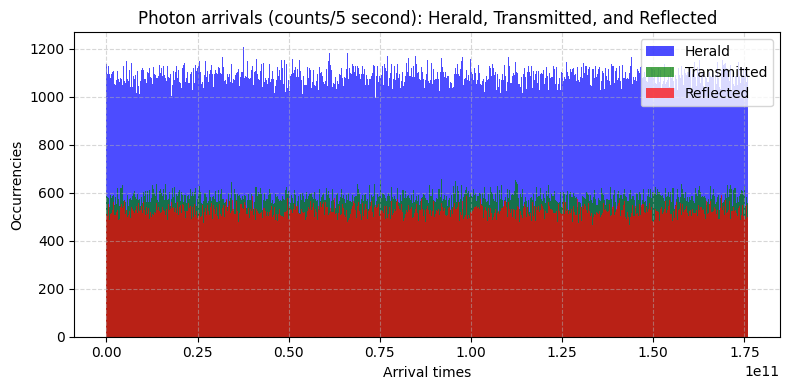
\includegraphics[width=\linewidth]{Images/photon_arrivals.png}
    \caption{Herald, transmitted, reflected photons arrival times (representing counts/5sec).}
    \label{fig:photon_arrivals}
\end{figure}

In order to proceed with the analysis, we need to take into account the herald photons, which are our control to see whether a couple of photon has been produced; thus, we need to analyze the time-stamps from the time tagger and search for simultaneous events. Depending on how simultaneous events are defined, we obtain different results, so it's necessary to choose a correct window over which consider events simultaneous: a window too large makes us lose any knowledge about near zero values (which are the most interesting) and a window too little could leave out too many events, not providing a significant statistic.
For this analysis I choose a window of $\Delta T = 50 \: mu \approx 4 \: ns$, which seems a reasonable value for simultaneous events (taking into account the different path lengths for herald and transmitted/reflected photon). Thus, analyzing the delay distributions between the transmitted/reflected photon and the nearest herald photon (within the window), we get the histograms in Figure~\ref{fig:delay_distributions}. As we can see, the histogram of the delay between Channel 1 and 2 (Herald and Transmitted) is peaked around zero (or small negative values), while the histogram of the delay between Channel 1 and 3 (Herald and Reflected) is peaked around positive values; this, again, is due to the different path lengths that the different photons have to walk in the experimental setup previously presented. Moreover, we see a significative difference in amplitude between the two distributions (and also in width): this is probably due to the beam splitter not being a perfect 50:50 beam splitter, which, for the total time of detection, accounts for a higher number of transmitted photons (about 10\% more frequent). In order to perform a better analysis we proceed to a normalization of these distributions and then a fit with a normal distribution; this is done because these delay distributions tend to be Gaussian due to a combination of factors:
\begin{itemize}
    \item Uncertainty in emission times: even though SPDC photons are generated simultaneously in theory, small fluctuations in the crystal and environmental conditions (e.g., temperature) can introduce slight variations in emission timing,  which can cause slight random shifts in the time-of-arrival of the herald and transmitted photons.
    \item Detector timing jitter: photodetectors have an inherent timing uncertainty, or jitter, which refers to random fluctuations in the exact moment a photon detection is registered. This jitter adds Gaussian noise to the time difference measurements, further contributing to a normal distribution of delays.
    \item Central Limit Theorem: since the total delay is influenced by multiple independent, small, random factors, the Central Limit Theorem applies. This theorem suggests that the sum of many independent random variables will approximate a normal distribution, even if the individual sources of variation are not perfectly Gaussian themselves.
\end{itemize}


\begin{figure}
    \centering
    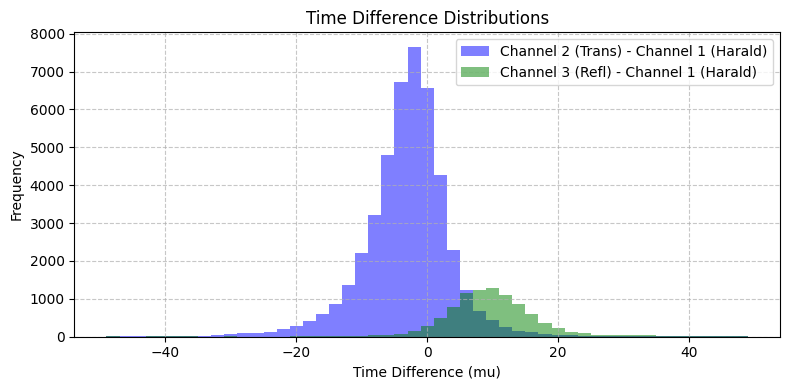
\includegraphics[width=\linewidth]{Images/delay_distributions.png}
    \caption{Delay distributions between Channels 1 and 2 and between Channels 1 and 3.}
    \label{fig:delay_distributions}
\end{figure}

\begin{figure}
    \centering
    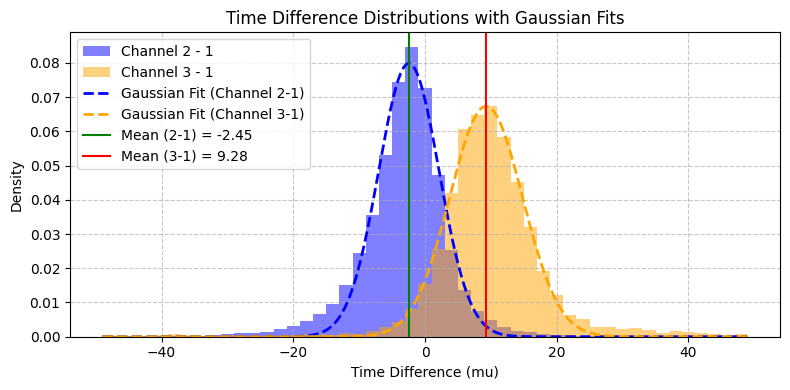
\includegraphics[width=\linewidth]{Images/delay_fit.png}
    \caption{Delay distributions with normal fits.}
    \label{fig:delay_fit}
\end{figure}

The result of these procedure is shown in Figure~\ref{fig:delay_fit}; the two distributions resemble normal distribution and both fit yield a good value of the RMSE ($0.0231$ for Trasmitted-Herald and $0.0213$ for Reflected-Herald). Table~\ref{tab:numerical} and Table~\ref{tab:fit} report the values of the mean and the standard deviation (related to the width of the bell), computed numerically and from the best parameter of the fit (respectively).
%
\begin{table}[b!]
    \centering
    \begin{tabular}{|c||c||c|}
        \hline
        \textbf{Statistic} & \textbf{Mean ($\mu$)} & \textbf{Std ($\mu$)} \\
        \hline
        \hline
        Channels 2 - 1 & -3.48 $\pm$ 0.03 & 6.99 $\pm$ 0.02 \\
        \hline
        Channels 3 - 1 & 9.30 $\pm$ 0.09 & 9.01 $\pm$ 0.07 \\
        \hline
    \end{tabular}
    \caption{Numerical Statistics}
    \label{tab:numerical}
\end{table}
%
\begin{table}[b!]
    \centering
    \begin{tabular}{|c||c||c|}
        \hline
        \textbf{Channel Pair} & \textbf{Mean ($\mu$)} & \textbf{Std ($\mu$)} \\
        \hline
        \hline
        Channels 2 - 1 & -2.45 $\pm$ 0.10 & 4.59 $\pm$ 0.10 \\
        \hline
        Channels 3 - 1 & 9.28 $\pm$ 0.07 & 5.52 $\pm$ 0.07 \\
        \hline
    \end{tabular}
    \caption{Fit Statistics}
    \label{tab:fit}
\end{table}

These values are not perfectly in agreement with each other, so it's necessary to spend some time commenting them, to better highlight where possible differences may arise: 
\begin{itemize}
    \item \textbf{Transmitted delay distribution:} Both numerically and with the fit we obtain a very similar value for the mean. On the other hand, the standard deviation computed numerically is about twice the one obtained from the fit: this is probably due to the fact that the the tails in the histogram are fatter than expected, which increases the deviation from the mean value.
    \item \textbf{Reflected delay distribution:} In this case we have a better agreement, with some differences both in the mean and in the standard deviation. In this case the problem is probably due to the low statistic, which doesn't make the distribution a perfect normal.
\end{itemize}
%
In both cases, an higher number of occurrences would make these distributions more significant and provide a better agreement with the fit. Moreover, a different choice for the simultaneous events window would modify the population of the tails, providing a more accurate standard deviation. 

The last point of the analysis is computing the value of $\alpha$, defined in Equation~\eqref{eq:alpha}. Table~\ref{tab:coincidences} reports the number of double and triple coincidences registered in the experiment. As we can see, the number of double coincidences between transmitted and reflected and the number of triple coincidences are really small w.r.t. the total of counts (respectively, 0.012 \textperthousand \: and 0.080 \textperthousand); this is in agreement with what expected (they should be zero) and these occurrences are probably due to some electrical noise or external photon and are not relevant. If we then apply Equation~\eqref{eq:alpha}, we get $\alpha = 0.00063 \pm  0.00005$, where the relative error is obtained taking the quadrature sum of the errors over the detection probabilities. This value is perfectly in line with what expected: we have proven that we are working in a quantum environment and that photons are indeed indivisible (as the coincidence probability between transmitted and reflected is negligible).

\begin{table}[!t]
    \centering
    \begin{tabular}{|l||c|}
        \hline
        \textbf{Type of Coincidence} & \textbf{Count} \\
        \hline
        \hline
        Triple Coincidences & 26 \\
        \hline
        Double Coincidences (H-T) & 45180 \\
        \hline
        Double Coincidences (H-R) & 9498 \\
        \hline
        Double Coincidences (T-R) & 175 \\
        \hline
    \end{tabular}
    \caption{Coincidence Counts}
    \label{tab:coincidences}
\end{table}


\subsection{Quantum random number generator}
\begin{figure}[!b]
    \centering
    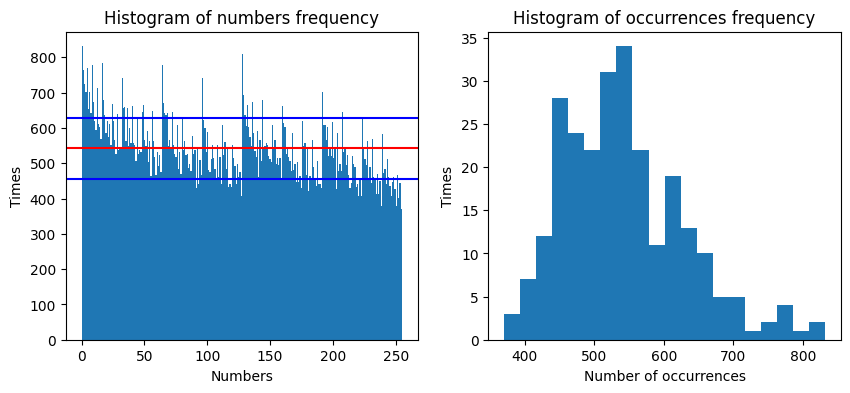
\includegraphics[width=\linewidth]{Images/qrng_stats.png}
    \caption{Quantum random number sequence analysis.}
    \label{fig:qrng_stats}
\end{figure}

\begin{figure}[!b]
    \centering
    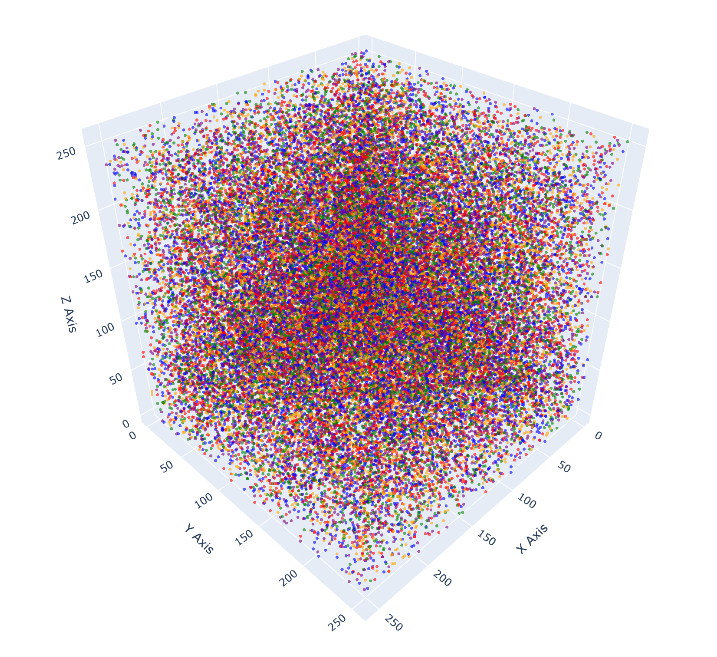
\includegraphics[width=\linewidth]{Images/QRNG.png}
    \caption{Cloud of points, generated using the QRN sequence from the experiment.}
    \label{fig:QRNG}
\end{figure}

The quantum random number generator is based on a quantum random number list, which can be obtained following the basic ideas explained in Section~\ref{sec:qrng_theory}. After building the bits list, grouping it into bytes and then transforming to decimal, we can analyze it in order to see whether it is really completely random or not. Figure~\ref{fig:qrng_stats} illustrates two histograms. The first histogram displays the frequency of each decimal number in the dataset, while the second histogram represents the occurrences of these frequencies, showing how many times each frequency value appears in the first histogram. From these histograms, we can see that the number distribution is pretty not very uniform, presenting some unexpected periodic peaks (even if the mean is $120.81$, which is near the expected value); on the other hand the occurrences distribution is peaked around the middle, with low-population tails, as expected. 

This is the first step in order to see if the QRNG is working correctly; we can visualize it also in 3D (considering the numbers in triplets, simulating 3D coordinates), as in Figure~\ref{fig:QRNG}. The cloud is dense and doesn't present any visible pattern, which is another point in favour of our thesis (also rotating it nothing strange appears, nothing related to the periodic peaks previously highlighted). 

But how can we be sure that this sequence is truly random? We need to investigate more in order to understand if our quantum random number list is truly random or has some intrinsic correlation. In order to do so, we leverage some statistical methods developed to study the randomness of a number sequence, based on the ENT module (see Appendix~\ref{sec:appendix_random}). When we apply these method to our quantum random number sequence, the output we get is:

\begin{enumerate}
    \item \texttt{Entropy: 0.998025 bits per bit.}
    \item \texttt{Optimum compression would reduce the size of this 1109816 bit file by 0 percent.}
    \item \texttt{Chi-square distribution for 1109816 samples: 3037.41, randomly exceeding this value 0.01 percent of the time.}
    \item \texttt{Arithmetic mean value of data bits: 0.4738 (0.5 = random).}
    \item \texttt{Monte Carlo value for Pi: 3.287920073 (error 4.66 percent).}
    \item \texttt{Serial correlation coefficient: 0.013837 (totally uncorrelated = 0.0).}
\end{enumerate}

On the other hand, when applied to a pseudo-random number sequence (using the \texttt{numpy.random} module), the output we get is:
\begin{enumerate}
    \item \texttt{Entropy: 0.337119 bits per bit.}
    \item \texttt{Optimum compression would reduce the size of this 9067776 bit file by 66 percent.}
    \item \texttt{Chi-square distribution for 9067776 samples: 6943909.07, randomly exceeding this value less than 0.01 percent of the time.}
    \item \texttt{Arithmetic mean value of data bits: 0.0625 (0.5 = random).}
    \item \texttt{Monte Carlo value for Pi: 4.000000000 (error 27.32 percent).}
    \item \texttt{Serial correlation coefficient: 0.400053 (totally uncorrelated = 0.0).}
\end{enumerate}

As we can clearly see, all the results for the quantum random number sequence suggest a high value of randomness, with near-zero correlation, while those obtained for the pseudo-random number sequence reveal the existence of an intrinsic correlation, which makes the sequence not truly random.

\section{Conclusions}
In this paper, we explored the functionality of a heralded single-photon source based on Spontaneous Parametric Down-Conversion (SPDC) and its performance within the context of the GRA experiment. The experimental results verify Malus’ law, highlighting the robust fit of the transmission model for polarized photons, with an RMSE of 0.4\%; the extracted fit parameters $b$ and $c$, essential for our setup, demonstrate excellent alignment with theoretical expectations.

Furthermore, we analyzed the delay distributions between herald and transmitted/reflected photons; numerical and fit results for delay distributions were consistent, though slight discrepancies can be attributed to the influence of the detection setup, particularly the beam splitter’s performance, and low detection counts in some cases. The numerically and fit-derived standard deviations confirm that the timing resolution falls within the anticipated noise range. It has been highlighted that having more statistic for both cases would provide a better agreement between the fit and the numerical statistics.

Finally, we examined the performance of a quantum random number generator (QRNG) based on our photon detection data. Statistical analysis of the generated sequence showed high entropy, minimal serial correlation, and good alignment with the expected randomness criteria, in contrast to results from a pseudo-random sequence. This supports the hypothesis that the QRNG based on quantum phenomena exhibits true randomness, suitable for secure cryptographic applications.

Our findings confirm that the SPDC source, combined with the heralded detection setup, provides a reliable single-photon source, exhibiting the non-classical behavior necessary for advanced quantum experiments (as proved by the value of $alpha$, which is well under the classical threshold).


\section{Appendix}
\subsection{Statistical methods for randomness analysis}
\label{sec:appendix_random}
The statistical methods to study the randomness of a number sequence are based on the ENT module, which is a ``Pseudorandom Number Sequence Test Program"~\cite{fourmilab}. Here we'll explain the main principle of each method, highlighting good and bad results. 

\begin{itemize}
    \item \textbf{Entropy}: Measure of the information density in a sequence of data (often expressed in bits per character or bits per symbol), it quantifies the unpredictability or randomness of a sequence, with higher entropy corresponding to a higher degree of randomness. The formula for entropy $H$ is:
    %
    \begin{equation}
        H = -\sum_{i=1}^{n} p_i \log_2 p_i
    \end{equation}
    %
    where $p_i$ is the probability of occurrence of the $i$-th symbol in the sequence. Entropy close to the theoretical maximum indicates that the data is highly random, while lower entropy suggests a more structured or predictable sequence.

    \item \textbf{Chi-Square Test}: Statistical method used to assess whether the distribution of elements in a data sequence deviates from what would be expected in a random sequence. It compares the observed frequencies of data points to the expected frequencies under the assumption of uniform randomness. The chi-square statistic is given by:
    %
    \begin{equation}
        \chi^2 = \sum_{i=1}^{k} \frac{(O_i - E_i)^2}{E_i}
    \end{equation}
    %
    where $O_i$ is the observed frequency of the $i$-th event and $E_i$ is the expected frequency. The result of the test can be expressed as a percentage, indicating the probability that the observed distribution could arise from a truly random process: values far from 50\% suggest non-randomness.

    \item \textbf{Arithmetic Mean}: Basic statistical measure that computes the average value of all the bytes (or bits) in a sequence; for a truly random sequence, the mean should be approximately 127.5 when considering bytes (ranging from 0 to 255) or 0.5 when considering bits (0 or 1). Deviations from the expected mean can indicate systematic biases or non-randomness.

    \item \textbf{Monte Carlo Method for Pi}: This method utilizes randomly generated data to estimate the value of $\pi$. Each successive sequence of six bytes (or other length of interest) is treated as coordinates $(x, y)$ within a square, and the fraction of points falling inside the inscribed circle is used to approximate $\pi$. The value of $\pi$ is approximated as:
    %
    \begin{equation}
        \pi \approx 4 \times \frac{\text{number of points inside the circle}}{\text{total number of points}}
    \end{equation}
    %
    For sufficiently large data sets, the approximation converges to the true value of $\pi$ only if the data is random.

    \item \textbf{Serial Correlation Coefficient}: Measures the extent to which each value in a sequence is related to its predecessor and is calculated as:
    %
    \begin{equation}
        \rho = \frac{\sum_{i=1}^{N-1} (x_i - \mu)(x_{i+1} - \mu)}{\sum_{i=1}^{N} (x_i - \mu)^2}
    \end{equation}
    %
    where $x_i$ are the data points, $\mu$ is the mean of the sequence, and $N$ is the total number of points.  For a random sequence, this correlation should be close to zero, indicating no dependence between consecutive elements; on the other hand, a coefficient close to 1 or -1 indicates strong correlation (or anti-correlation), which suggests the sequence is not random.
\end{itemize}

\section{Code}
All the data and the code for the data analysis can be found in this public Github repository: \href{https://github.com/Kallo27/QOL/tree/main/Lab2}{https://github.com/Kallo27/QOL/tree/main/Lab2}

\begin{thebibliography}{99}

\bibitem{pap1}
  P. Grangier, G. Roger and A. Aspect, \textit{Experimental Evidence for a Photon Anticorrelation Effect on a Beam Splitter: A New Light on Single-Photon Interferences}, Europhysics letters (1986).

\bibitem{pap2}
  E. Hecht, \textit{Optics}, 5th ed., Addison-Wesley (2017).
  
\bibitem{pap3}
  R. W. Boyd, \textit{Nonlinear Optics}, Academic Press (2020).

\bibitem{fourmilab}
  J. Walker, \textit{HotBits: Genuine Random Numbers from Radioactive Decay}, \href{https://www.fourmilab.ch/random/}{https://www.fourmilab.ch/random/}.

\end{thebibliography}

\end{document}
